%latex model.tex
%bibtex model
%latex model.tex
%latex model.tex
%dvipdfm model.dvi

%se poate lucra si online (de ex www.overleaf.com)


\documentclass[runningheads,a4paper,11pt]{report}

\usepackage{algorithmic}
\usepackage{algorithm}
\usepackage{array}
\usepackage{amsmath}
\usepackage{amsfonts}
\usepackage{amssymb}
\usepackage{amsthm}
\usepackage{caption}
\usepackage{comment}
\usepackage{epsfig}
\usepackage{fancyhdr}
\usepackage[T1]{fontenc}
\usepackage{geometry}
\usepackage{graphicx}
\usepackage[colorlinks]{hyperref}
\usepackage[latin1]{inputenc}
\usepackage{longtable}
\usepackage{multicol}
\usepackage{multirow}
\usepackage{rotating}
\usepackage{setspace}
\usepackage{subfigure}
\usepackage{url}
\usepackage{verbatim}
\usepackage{xcolor}

\geometry{a4paper,top=3cm,left=2cm,right=2cm,bottom=3cm}

\pagestyle{fancy}
\fancyhf{}
\fancyhead[LE,RO]{Authentication based on face recognition for preschoolers}
\fancyhead[RE,LO]{Team06}
\fancyfoot[RE,LO]{ITSG 2019-2020}
\fancyfoot[LE,RO]{\thepage}

\renewcommand{\headrulewidth}{2pt}
\renewcommand{\footrulewidth}{1pt}
\renewcommand{\headrule}{\hbox to\headwidth{%
\color{lime}\leaders\hrule height \headrulewidth\hfill}}
\renewcommand{\footrule}{\hbox to\headwidth{%
\color{lime}\leaders\hrule height \footrulewidth\hfill}}

\hypersetup{
pdftitle={artTitle},
pdfauthor={name},
pdfkeywords={pdf, latex, tex, ps2pdf, dvipdfm, pdflatex},
bookmarksnumbered,
pdfstartview={FitH},
colorlinks=true,
citecolor=green,
}
% \pagestyle{plain}

\setcounter{secnumdepth}{3}
\setcounter{tocdepth}{3}

\linespread{1}

% \pagestyle{myheadings}

\makeindex


\begin{document}

    \begin{titlepage}
        \sloppy
        \begin{center}
            BABE\c S BOLYAI UNIVERSITY, CLUJ NAPOCA, ROM\^ ANIA

            FACULTY OF MATHEMATICS AND COMPUTER SCIENCE

            \vspace{6cm}

            \Huge \textbf{Authentication based on face recognition for preschoolers}

            \vspace{1cm}

            \normalsize -- ITSG report --

        \end{center}


        \vspace{5cm}

        \begin{flushright}
            \Large{\textbf{Team members}}\\
            Truta Diana, 258 \\
            Vlad Cristina, 258 \\
            Turean Christine, 258 \\
            Igna Darius, 258 \\

        \end{flushright}

        \vspace{4cm}

        \begin{center}
            2019
        \end{center}

    \end{titlepage}

    \pagenumbering{gobble}

    \begin{abstract}
        Nowadays technology is everywhere. Children interact all day with different applications.They are a special category of humans with low or none abilities of writing and reading therefore a login with facial recognition is needed. We aim to solve this problem. Our approach involves using OpenCV face recognition for children authentication. We made a comparison regarding algorithm performance between adult faces data and preschoolers faces data before and after tuning some parameters of the algorithm.
    \end{abstract}


    \tableofwcontents

    \newpage

    \listoftables
    \listoffigures

    \newpage

    \setstretch{1.5}



    \newpage

    \pagenumbering{arabic}





    \chapter{Introduction}
    \label{chapter:introduction}

    \section{What? Why? How?}
    \label{section:what}

    Face recognition, as one of the most successful applications of image analysis, has recently gained significant attention from the scientific world. This happened due to the technologies development and the necessity to automate different tasks. Since the 1960s, the research in automatic face recognition has had a big evolution, but many of the problems in this area are unsolved. In addition, reliable face recognition still offers a great challenge to computer vision and pattern recognition researchers. The main reasons for the recent increased interest in face recognition study field are represented by the need for identity verification in the digital world, public concern about security and also the face analysis and modelling techniques used in multimedia data management and computer entertainment.



    \section{Paper structure and original contribution(s)}
    \label{section:structure}
    The paper is structured in 6 chapters which describe our experimental study during the last months. The introduction presents the general approach for the face recognition issue, this being continued with the problem statement that describes the actual problem we were trying to solve. Moreover, the state of the art part exposes the techniques used in different papers and their obtained results. Our proposed approach is presented in chapter 4 along with the method used and its description.The next chapter presents the results based on the developed application. The last part, chapter 6, summarizes the problem statement, presents our perspective and the future work we are considering to do.
    Our original contribution is represented by the comparison done between two different approaches that are presented below in the paper.

    \chapter{Scientific Problem}
    \label{section:scientificProblem}


    \section{Problem definition}
    \label{section:problemDefinition}
    Nowadays almost all applications require authentication of the user. The most popular authentication method is face recognition. When talking about kids the necessity of this authentication comes from the fact that the preschoolers cannot read or write in order to get authenticated, so face recognition can be a solution to this problem. In addition, this problem is very frequent mainly because nowadays preschoolers have access to many applications that require authentication, so the face recognition mechanism would help them log in.
    We are trying to build an application in which the children can login with facial recognition.



    \chapter{State of art/Related work}
    \label{chapter:stateOfArt}

    Face recognition represents a subject of interest in the domain of Artificial Intelligence and some studies revealed important results when considering the Convolutional Neural Networks \cite{hu2015face}. The paper compares different types of CNNs and shows the results of their experiments, considering different architectures and configurations (CNN-S, CNN-M, CNN-L). CNN-S and and CNN-M have 3 convolutional layers and two fully connected layers, but CNN-M has more filters than CNN-S. In contrast with these two, CNN-L has 4 convolutional layers. In addition, softmax was used in the last layer for predicting one of K mutually exclusive classes. During the training phase, the learning rate was set to 0.001 for all the three networks and the batch size was fixed to 100. For the database, it was used LFW that contained 5.749 subjects and 13.233 images. The computed accuracy shows a value of 0.7828 for CNN-S, 0.7882 for CNN-M and 0.7807 for CNN-L. These values highlighted the fact that CNN-M achieves the best face recognition performance when applied on the LFW data. In addition, one of the conclusions is that fusion of features from different CNN layers increase the performance of the network. This is why, CNNs have achieved very good results in face recognition problems recently.

    Singh, Shilpi, and S. V. A. V. Prasad wrote a comprehensive and complex study about face recognition subject: ''Techniques and Challenges of Face Recognition: A Critical Review.''\cite{singh2018techniques} . In this paper there are presented the main challenges researchers encounter when dealing with face recognition : aligning, thermal image, iris, occlusion, facial expressions ,poses and facial advances. They also discuss about the three types of face recognition, namely 2D, 2D-3D and 3D. In their comparison we can see that ''Improving face recognition with domain adaptation'' \cite{wen2018improving} achieved the highest accuracy of 99.33\% for face recognition of wild animal tested on LFW dataset with domain adaptation technique . Another high accuracy rate of 99.07\%  was achieved using Fusion algorithm \cite{seal2016human} or RF classifiers for human face which was tested on UGC-JU face database.

    Other methods used to solve this problem are: Histogram Oriented Gradient(HOG)\cite{fathi2016new}, Multi-scale strategy based on geometric and local descriptors \cite{zhou2018pose}, local geometric feature and shape matching \cite{guo2016ei3d}, face descriptor based on Gabor filter \cite{aksasse2017novel}. Database used by researchers presented in this paper are : ORL , YALE, PHPID, VLC, GAVAbDB, AR, UGC-JU, CURTIN, FRGC, Bosphorous, LFW database.

    Many research papers used the conventional pipeline that consists of four stages: detect => align => represent => classify. Taigman, Yaniv, et al revised this pipeline, both the alignment step and the representation step, in ''Deepface: Closing the gap to human-level performance in face verification.'' \cite{taigman2014deepface}  by employing explicit 3D face modeling in order to apply a piecewise affine transformation, and derive a face representation from a nine-layer deep neural network Fig. \ref{img1}. In alignment step they get rid of variation within the face images, so that every face seems to look straight into the camera (''frontalized'').They trained their network on the Social Face Classification (SFC) dataset(i.e. not public) They tested their approach on LFW dataset with 94.3\% mean accuracy on face recognition and 97.25\% mean accuracy on face verification.

    \begin{figure}[!htb]
        \centering
        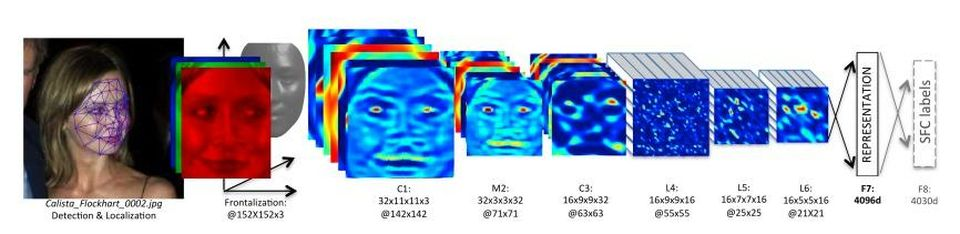
\includegraphics[scale=0.45]{Figures/img1.jpg}
        \caption{Visualization of the architecture of proposed method in \cite{taigman2014deepface}}
        \label{img1}
    \end{figure}

    Lu, Chaochao, and Xiaoou Tang propose in ''Surpassing human-level face verification performance on LFW with GaussianFace.'' \cite{lu2015surpassing}  a principled multi-task learning approach based on Discriminative Gaussian Process Latent Variable Model (DGPLVM), named GaussianFace, for face verification. They also use the low rank approximation method to speed up the process of inference and prediction. They obtained an accuracy rate of 98.52\% on Labeled Faces in the Wild (LFW) benchmark.

    In order to recognise human emotion, Tarnowski, Paweł, et al propose a new approach in ''Emotion recognition using facial expressions.'' \cite{tarnowski2017emotion} . They divide emotions in seven groups  (neutral, joy, sadness, surprise, anger, fear, disgust) based on facial expressions.The classification of features were performed using k-NN (3-NN) classifier and MLP neural network (two-layer neural network classifier, with 7 neurons in the hidden layer ). For testing their approach they build their own data and adopt two ways: subject-dependent - for each user separately and subject-independent - for all users together. In both cases, for 3-NN classifier, data were randomly divided on the teaching part (70\%) and the testing part (30\%) and for MLP into three groups: teaching (70\%), testing (15\%) and validation (15\%).


    \chapter{Proposed approach}
    \label{chapter:proposedApproach}

    For face recognition we used the proposed solution from OpenCv. Their approach is based on deep metric learning. Instead, of trying to output a single label, whether person X is in the image, they output a real-valued feature vector. In the figure \ref{img2} we have illustrated the overview of the pipeline proposed by the scientists from OpenCV for fac.

    \begin{figure}[!htb]
        \centering
        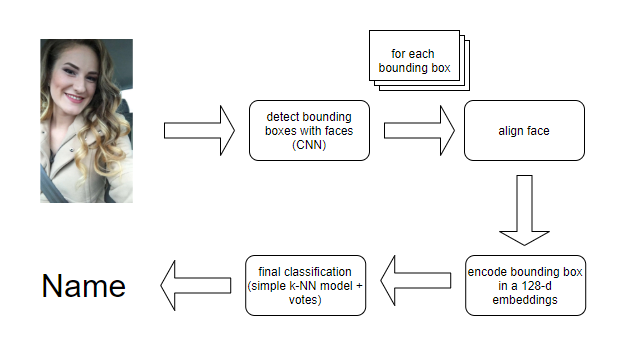
\includegraphics[scale=0.9]{Figures/img2.png}
        \caption{Overview of the OpenCV face recognition pipeline}
        \label{img2}
    \end{figure}

    For the input image, using a CNN, all faces are detected and bounding boxes are extracted from the original image. At this stage it is used a ResNet-34 from the Deep Residual Learning for Image Recognition \cite{he2016deep} paper by He et al., but with fewer layers (29 conv layers) and numbers of filters reduced by half. Next each bounding box is wrap so that the eyes and lips are always in the same place in the image. Using this transformation will reduce the examples that need to be learned and will make it a lot easier to compare faces in the next steps.
    To make the necessary transformation it is used an algorithm called face landmark estimation, namely, the approach proposed by Vadih Kazemi and Josephine Sullivan ''One millisecond face alignment with an ensemble of regression trees'' \cite{kazemi2014one}.

    Next step is to take each bounding box which was detected at previous step and encode in 128 numbers. This is done by training a Deep Convolutional Neural Network to generate 128 measurements.

    \begin{figure}[!htb]
        \centering
        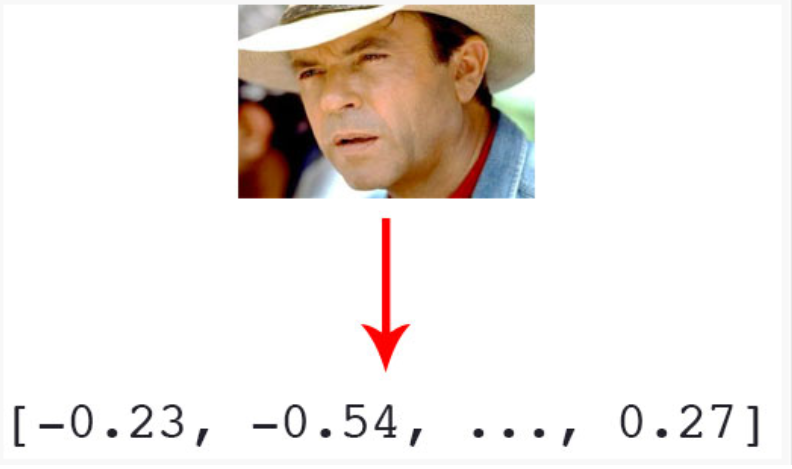
\includegraphics[scale=0.6]{Figures/img4.png}
        \caption{ Generation a 128-d real-valued number feature vector per face \cite{binotuopencv}}
        \label{img4}
    \end{figure}

    The training process for encoding phase works by looking at 3 face images at a time, two images with the same person and the third one with a different person. Then the algorithm looks at the measurements it is currently generating for each of those images. The parameters of the network are slightly tweak so that it makes sure the measurements it generates for the images with the same person are closer while making sure the measurements for the third image are further apart from the other two.In the Figure \ref{img3} we have presented a simplified example of training step.

    \begin{figure}[!htb]
        \centering
        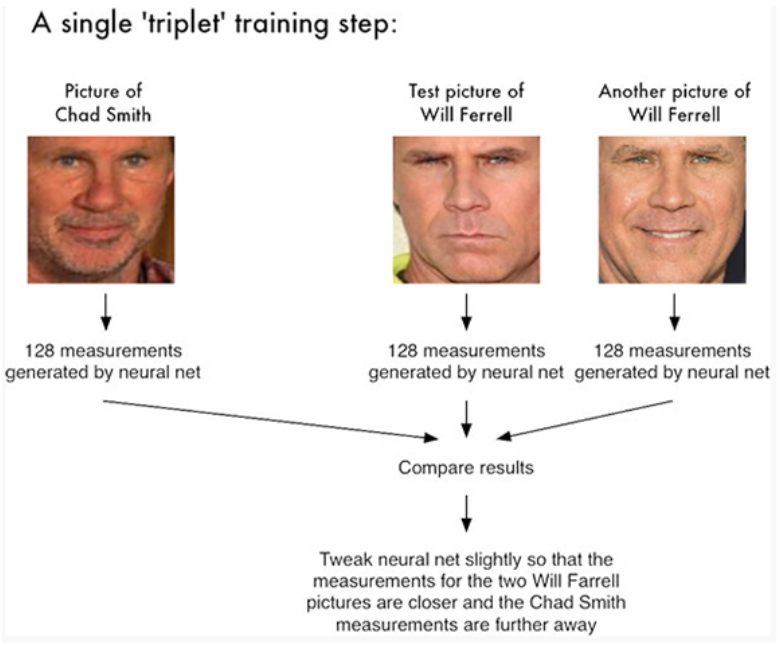
\includegraphics[scale=0.6]{Figures/img3.png}
        \caption{ The triplet training step consists of two images of the same person and another image of a different person. The neural network generates a 128-d vector for each of the three images. The neural network weights are tweak to make the two vectors of the same person closer via distance metric.\cite{binotuopencv}}
        \label{img3}
    \end{figure}

    The team from OpenFace[15] published several trained networks which are ready to use for embedding proposals. Which is our case, for this step of the approach it is used a pre-trained network from OpenFace.
    After the encoding of 128 vector is obtained then at the training phase these vectors are saved for every person in order to form the dataset of ''known'' users.
    In the last step of classification of a face , using the embedding a k-NN model with votes is applied.

    We integrated the face recognition model into a web application which offers login functionality to the user. From the business point of view, we provide different screens to the user (child or teacher). After login, the child enters a screen where a game should start. If the logged in user is a teacher, then he/she will be able to add a new child to the system in order for him to be able to play the game.

    Considering the technical part of our approach, we used a server designated to process requests for classifying an image. This server is implemented in Python. It communicates via REST calls with the Java app. The Java application is responsible of maintaining the database and provide the following functionalities to the user: log in, add user to the system. From the architectural point of view, the application has a layered client-server architecture with the following layers: client, core, repository and test. The client component keeps the displays for the user, the core can be seen as a service (processing calls from the client to the repository component). The repository is responsible of communicating with the database, while the test component, as the name suggests has tests.

    \chapter{Application (numerical validation)}
    \label{chapter:application}


    \section{Methodology}
    \label{section:methodology}

    For evaluating the face recognition method we looked into some metrics like accuracy, time, complexity. The accuracy test if our classification model does the right predictions. We also evaluate the time used for generating classifications and the complexity of the method and the used tools.
    The experiment tested if our face recognition model would correctly recognize a new face and label it with the correct person name or id.
    The independent variable in the process is the face image and the dependent variable is the person name prediction. In order to correctly validate the system we used some real data containing raw labeled face images collected from the web. The dataset is called ''Labeled faces in the wild''.For each person used in our experiment we split the images in train and test sets. We tested how accurate is the system in predicting a person name by using a new image of that person.


    \section{Data}
    \label{section:data}

    One used dataset contains images from ''Labeled faces in the wild''. From 1600 persons we used the persons that have more than 5 images. In the experiment we used 4910 images from 276 different persons. Many groups are not well represented in LFW dataset. For example, there are very few children, no babies, very few people over the age of 80, and a relatively small proportion of women. In addition, many ethnicities have very minor representation or none at all. All the data is collected from the web.

    Another used dataset contains images from the set of images provided by the kindergarten teacher. We built our dataset in the following way: used 10 children and captured 5 images per child on average. The dataset contains cropped photos of only their faces. In addition, some photos captured the children from the side. The total number of images gathered is 50. We wanted to test the classification equally on girls and boys, that is why we chose photos of 5 girls and 5 boys.

    \section{Results}
    \label{section:results}

    The algorithm has reached an accuracy of 95.28\% when using the improved version with face alignment of the OpenCV library: (see Table \ref{tab3PSO})


    \begin{longtable}[c]{ c | c | c | c | c | c }
        \caption{Comparison between the obtained results of the algorithm before and after improvement conducted on the photos of adult vs photos of children.}\label{tab3PSO}\\

        \hline
        \multirow{2}{4em}{} & \multicolumn{2}{c}{Algorithm without alignment } & \multicolumn{2}{|c|}{Algorithm with alignment} & \multirow{2}{11em}{Deep Residual Learning on ResNet-34} \\

        & Kids & Adults & Kids & Adults\\
        \hline\hline
        \endfirsthead
        \endhead

        \hline
        \endfoot

        \hline
        \hline\hline
        \endlastfoot

        Number of images & 50 & 4910 & 50 & 4910 & 3million \\
        Number of people & 10 & 276 & 10 & 276\\
        Matching tolerance & 0.6 & 0.6 & 0.5 & 0.5 \\
        \hline
        Accuracy & 30\% & 90\% & 64.74\% & 95.28\% & 99.38\%\\
    \end{longtable}

    As we can see, given the different sizes of the datasets (kids vs adults), the obtained results are distant from one another when evaluating the algorithm without alignment vs with alignment.

    \section{Discussion}
    \label{section:discussion}

    When comparing our results with the state-of-the-art methods, such as Deep Residual Learning on ResNet-34, our approach did not reach a better accuracy, but that we consider that our work was not in vain, since we managed to reach an accuracy close to the state-of-the-art.

    We consider that one weak spot of our approach was the limited dataset in the case of children. One solution to improve our performance would be to maybe use a larger dataset in which the focus remains on children, because the number of features extracted from children is smaller compared to adults.

    \chapter{Conclusion and future work}
    \label{chapter:concl}
    Face recognition is still a challenging problem in the field of computer vision. Moreover, it has received a lot of attention over the past decade because of its several applications that are practical in various domains. Although there are still many aspects that can be improved, face recognition systems are far from ideal to perform adequately in all situations imposed by a real environment.
    In addition, the research presented in this paper was applied on images with preschoolers faces which has made the entire process more difficult due to the fact that they do not have mature face features and many reseable each other.
    As future work, we would like to try other types of face recognition algorithms, such as Local Binary Patterns Histograms (LBPH) or deep learning, and to reach even better results.



    \bibliographystyle{plain}
    \bibliography{bib}

\end{document}